
\chapter{数形转换}
\label{chap:number-to-graph}

\section{方程与图形}
\label{sec:equation-and-graph}

\begin{example}
  已知实数$x,y$满足$2x+3y=6$,求$xy$的最大值。
\end{example}
\begin{proof}[提示]
  此类问题的常见的方法是换元求二次方程最大最小值。如果结合图形考虑,如在笛卡尔坐标下,则
  \begin{align*}
    2x+3y=6
  \end{align*}
  是一条直线,而$xy$则是面积(不考虑符号),如图。
  
  \begin{center}
    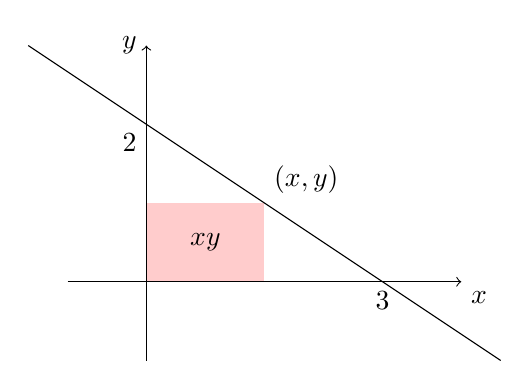
\begin{tikzpicture}[scale=1.0]
      \coordinate[label=above right:${(x,y)}$] (A) at(1.5,1);
      \coordinate[label=below left:2](B) at (0,2);
      \coordinate[label=below:3](C) at (3,0);

      \fill[color=red!20](0,0) rectangle(A) node[midway]{$xy$};
      \node at(0.75,0.5) {$xy$};
      \draw[->](-1,0)--(4,0) node[below right]{$x$};
      \draw[->](0,-1)--(0,3) node[left]{$y$};
      \draw(-1.5,3)--(4.5,-1);
      \tkzDrawPoints(A,B,C)
    \end{tikzpicture}
  \end{center}  

  显然,$xy$只能在直线$2x+3y=6$落于第一象限的部分内取得最大值,因为其它象限直线上的点与原点组成的矩形面积$xy$是“负”的。原问题与下面的几何问题等价:

  直角边长分别为2和3的直角三角形,在斜边上任取一点向两直角边作垂线,求两垂线与直角边构成的矩形面积最大时该点的位置。
\end{proof}

\begin{example}
  先特殊化,等腰直角三角形斜边上任取一点,求对应矩形面积取得最大值时该点的位置。
\end{example}
\begin{proof}[提示]
  直觉上应该是斜边的中点\footnote{数学上直觉很重要。}。这里猜不出来也不要紧,可以想象一下,在顶点的时候,面积是零,所以从顶点出发往中间走的时候,面积是增加的。又由于两个顶点其实是对称的,想象两个动点以相同的速度分别从两个顶点往中间出发,面积都是增加的,当两个动点在斜边的中点相遇的时候,面积应该就是最大值。

  \begin{center}
    \begin{tikzpicture}[scale=1.0]
      \begin{scope}[shift={(0,0)}]
        \coordinate(O)at(0,0);
        \coordinate(A)at(4,0);
        \coordinate(B)at(0,4);
        \coordinate(C)at(2,2);
        \coordinate(Cx)at(2,0);
        \coordinate(Cy)at(0,2);
        
        \coordinate(D)at(2.5,1.5);
        \coordinate(E)at(1.5,2.5);
        \fill[color=red!10](O)rectangle(C);
        \draw(O)--(A)--(B)--cycle;
        \draw(Cx)--(C)--(Cy);
        \tkzDrawPoints(C)
      \end{scope}
      \begin{scope}[shift={(4.5,0)}]
        \coordinate(O)at(0,0);
        \coordinate(A)at(4,0);
        \coordinate(B)at(0,4);
        \coordinate(C)at(2,2);
        \coordinate(Cx)at(2,0);
        \coordinate(Cy)at(0,2);
        \coordinate(D)at(1.5,2.5);
        \coordinate(Dx)at(1.5,0);
        \coordinate(Dy)at(0,2.5);
        %\fill[color=red!10](O)rectangle(C);
        \fill[color=red!10](C)--(D)--(Dx)--(Cx)--cycle;
        \fill[pattern=north east lines](C)--(D)--(Dy)--(Cy)--cycle;
        \draw[dashed](Cx)--(C)--(Cy);
        \draw(Dx)--(D)--(Dy);
        \draw(O)--(A)--(B)--cycle;
        \tkzDrawPoints(C)
      \end{scope}
      \begin{scope}[shift={(9,0)}]
        \coordinate(O)at(0,0);
        \coordinate(A)at(4,0);
        \coordinate(B)at(0,4);
        \coordinate(C)at(2,2);
        \coordinate(Cx)at(2,0);
        \coordinate(Cy)at(0,2);
        \coordinate(D)at(1.5,2.5);
        \coordinate(Dx)at(1.5,0);
        \coordinate(Dy)at(0,2.5);
        \coordinate(E)at(2.5,1.5);
        \coordinate(Ey)at(0,1.5);
        % \fill[color=red!10](O)rectangle(C);
        \fill[color=red!10](C)--(E)--(Ey)--(Cy)--cycle;
        \fill[pattern=north east lines](C)--(D)--(Dy)--(Cy)--cycle;
        \draw[dashed](Cx)--(C)--(Cy) (E)--(Ey);
        \draw(Dx)--(D)--(Dy);
        \draw(O)--(A)--(B)--cycle;
        \tkzDrawPoints(C)
      \end{scope}
    \end{tikzpicture}
  \end{center}

  由图,可以看出,当动点离开中点时,面积是减小的(因为增加的面积小于减小的面积,从而面积净增量是负的,把第二图中的增加区域等价变换到第三图中的同等染色区域就很明显了)。也就是动点在斜边中点时,矩形面积达到最大,为等腰直角三角形的一半。

  \begin{center}
    \begin{tikzpicture}[scale=1.0]
      \coordinate(O)at(0,0);
      \coordinate(A)at(4,0);
      \coordinate(B)at(4,4);
      \coordinate(C)at(0,4);
      \coordinate(D)at(2,2);
      \coordinate(Dx1)at(2,0);
      \coordinate(Dx2)at(2,4);
      \coordinate(Dy1)at(0,2);
      \coordinate(Dy2)at(4,2);
      \coordinate(E)at(1.5,2.5);
      \fill[color=red!10](Dx1)--(D)--(Dy2)--++(0,0.5)--(E)--(1.5,0)--cycle;
      \fill[pattern=north east lines](D)--(Dx2)--++(-0.5,0)--(E)--(0,2.5)--(Dy1)--cycle;
      \draw(O)--(A)--(B)--(C)--cycle (A)--(C) (0,2)--(4,2) (2,0)--(2,4);
      \draw[dashed](1.5,0)--(1.5,4) (0,2.5)--(4,2.5);
      \tkzDrawPoints(D, E)
    \end{tikzpicture}
  \end{center}

  把等腰直角三角形补充为一个正方形,则更明显。当动点从中点移动时,减小的一圈是往外扩张(与$\frac14$个小正方形比)的,而增加的一圈则是往内收缩的,其面积大小是很明显的\footnote{实际上其面积差值是中间重叠部分的两倍。}。
\end{proof}

\begin{example}
  利用上面等腰直角三角形的结论,求满足$2x+3y=6$是$xy$的最大值。
\end{example}
\begin{proof}[提示]
  换元,使直线的斜率的绝对值为1,从而变换为等腰直角三角形。令$u\equiv2x, v\equiv3y$,则原问题变换为求满足$u+v=6$下的$uv/6$的最大值。$uv/6$取得最大值时$(u,v)$点与$uv$取得取大值时的$(u,v)$点是一致的,从而当$u=v=3$时,$uv/6=3\times3/6=1.5$为最大值。
\end{proof}

\section{图形变代数}
\label{sec:graph-to-algebra}

\begin{example}[2014 AMC12B 21]
  单位正方形$ABCD$中,矩形$JKHG$与$EBCF$全等。问$AE$的长度是多少?
  \begin{center}
    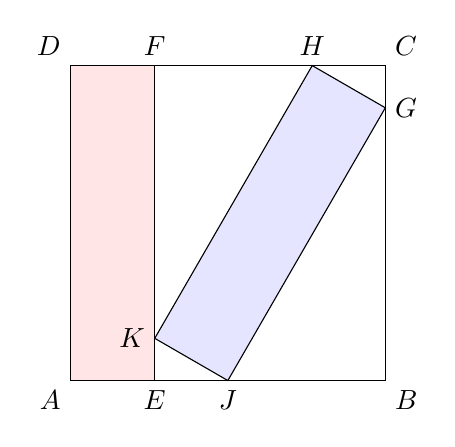
\begin{tikzpicture}[scale=1.0]
      \coordinate[label=below left:$A$](A)at(0,0);
      \coordinate[label=below right:$B$](B)at(4,0);
      \coordinate[label=above right:$C$](C)at(4,4);
      \coordinate[label=above left:$D$](D)at(0,4);

      \coordinate[label=below:$E$](E)at(1.0718, 0);
      \coordinate[label=above:$F$](F)at(1.0718, 4);
      \fill[color=red!10](A)--(E)--(F)--(D)--cycle;

      \coordinate[label=below:$J$](J)at(2, 0);
      \coordinate[label=left:$K$](K)at(1.0718, 0.536);
      \coordinate[label=above:$H$](H)at(3.0718, 4);
      \coordinate[label=right:$G$](G)at(4, 3.464);

      \filldraw[fill=blue!10](G)--(H)--(K)--(J)--cycle;

      \draw(A)--(B)--(C)--(D)--cycle;
      \draw(E)--(F);
    \end{tikzpicture}
  \end{center}
  \begin{align*}
    (A)\quad \frac12 (\sqrt6 - 2)\qquad
    (B)\quad \frac14             \qquad
    (C)\quad 2 - \sqrt3          \qquad
    (D)\quad \frac{\sqrt3}6      \qquad
    (E)\quad 1 - \frac{\sqrt2}2  \qquad
  \end{align*}
\end{example}
\begin{proof}[提示]
  第一种,使用几何方法,计算简单,但需要深刻的图形洞察力。$JG=AD=1$,猜测$J$是中点,则$BJ=0.5$,从而$\angle JGB=30^\circ$,剩余简单。

  第二种,设变量,导方程组,变换为含三角函数的代数运算。这种对图形洞察力的要求没那么高,但涉及的计算量有可能会非常复杂。
\end{proof}